\documentclass{beamer}
\usetheme{Antibes}
\usepackage{xcolor, colortbl}
\usepackage{algorithm}
\usepackage{algpseudocode}
\usepackage{textcomp}
\usepackage{listings}
\usepackage{hyperref}
\usepackage{alltt}
\usepackage{tikz}
\usepackage{framed}
\usepackage{marvosym}
\usepackage{wasysym}
\usepackage{marvosym}
\usepackage{crayola}
\usepackage{mathpartir}
\usepackage{tabularx}
\usepackage[belowskip=-15pt,aboveskip=0pt]{caption}
\usepackage[skins]{tcolorbox}
\usepackage{multicol}
\usetikzlibrary{positioning,shapes,arrows, backgrounds, fit, shadows, automata}
\usetikzlibrary{decorations.markings, calc}
%\usepackage{wasysym}
%\usepackage{marvosym}
\setbeamertemplate{footline}[frame number]
%\usecolortheme{fly}
\usefonttheme{serif}

\title[Sujit]{Lexical Analysis \\
Programming Languages}
\author{Sujit Kumar Chakrabarti}
\institute{IIITB}
\date{}


\definecolor{lightblue}{rgb}{0.8,0.93,1.0} % color values Red, Green, Blue
\definecolor{darkblue}{rgb}{0.4,0.3,1.0} % color values Red, Green, Blue
\definecolor{Blue}{rgb}{0,0,1.0} % color values Red, Green, Blue
\definecolor{darkgreen}{rgb}{0,0.7,0.2} % color values Red, Green, Blue
\definecolor{Red}{rgb}{1,0,0} % color values Red, Green, Blue
\definecolor{Pink}{rgb}{0.7,0,0.2}
\definecolor{links}{HTML}{2A1B81}
\definecolor{mydarkgreen}{HTML}{126215}
\newcommand{\highlight}[1]{{\color{Red}(#1)}}

\newcommand{\myheader}[1]{
	{\color{darkblue}
		\begin{Large}
			\begin{center}
				{#1}
			\end{center}
		\end{Large}
	}
}
\newcommand{\myminorheader}[1]{
	{\color{BrickRed}
		\begin{Large}
			{\fontfamily{\sfdefault}\selectfont\textbf{#1}}
		\end{Large}
	}
}

%\tikzstyle{input} = [coordinate]
%\tikzstyle{output} = [coordinate]


\tikzstyle{bb}=[%
      rectangle, draw=black, thick, fill=OliveGreen!30, drop shadow, align=center,
      text ragged, minimum height=2em, minimum width=2em, inner sep=6pt
]

\tikzstyle{inv}=[%
      rectangle, draw=none,  align=center,
      text ragged, minimum height=2em, minimum width=2em, align=center, inner sep=6pt
]

\tikzstyle{db}=[%
      ellipse, draw=black, thick, fill=pink, drop shadow, align=center,
      text ragged, minimum height=2em, inner sep=6pt
]

\tikzstyle{jn}=[%
      inner sep=0cm, outer sep=0cm
]

\tikzstyle{io}=[%
      trapezium, trapezium left angle=60, trapezium right angle=120, draw=black, thick, fill=brown, drop shadow,
      text ragged, minimum height=2em, minimum width=2em, inner sep=6pt, align=center
]

\tikzstyle{glio}=[%
      trapezium, trapezium left angle=60, trapezium right angle=120, draw=red, line width = 1mm, fill=brown, drop shadow,
      text ragged, minimum height=2em, minimum width=2em, inner sep=6pt
]
\tikzstyle{gl}=[%
      rectangle, draw=red, line width = 1mm, fill=lightblue, drop shadow,
      text ragged, minimum height=2em, minimum width=2em, inner sep=6pt
]

\tikzstyle{en}=[%
      rectangle, draw=black, thick, fill=none,
      text ragged, minimum height=2em, minimum width=2em, inner sep=6pt
]

\tikzstyle{sh}=[%
      rectangle, draw=gray, thick, fill=none, color = gray,
      text ragged, minimum height=2em, minimum width=2em, inner sep=6pt
]


\lstdefinestyle{javacode}{
	language = Java,
	basicstyle = \ttfamily\scriptsize,
	stringstyle = \ttfamily,
	keywordstyle=\color{Blue}\bfseries,
	identifierstyle=\color{Pink},
	commentstyle=\color{darkgreen},
	frame=single,
	frameround=tttt,
%	numbers=left
	showstringspaces=false
}

\lstdefinestyle{camlcode}{
	language = Caml,
	basicstyle = \scriptsize\ttfamily,
	stringstyle = \color{red}\ttfamily,
	keywordstyle=\color{Blue}\bfseries,
	identifierstyle=\ttfamily,
	frame=single,
	frameround=tttt,
	numbers=none,
	showstringspaces=false,
	escapeinside={(*@}{@*)}
}

\lstdefinestyle{outputcode}{
	language = bash,
	backgroundcolor = \color{black},
	basicstyle = \tiny\ttfamily\color{white},
	stringstyle = \color{red}\ttfamily,
	keywordstyle=\color{white}\bfseries,
	identifierstyle=\ttfamily,
	frameround=tttt,
	numbers=none,
	showstringspaces=false,
	escapeinside={(*@}{@*)}
}

\newtcolorbox{myframe}[2][]{%
  enhanced,colback=white,colframe=black,coltitle=black,
  sharp corners,boxrule=0.4pt,
  fonttitle=\itshape,
  attach boxed title to top left={yshift=-0.3\baselineskip-0.4pt,xshift=2mm},
  boxed title style={tile,size=minimal,left=0.5mm,right=0.5mm,
    colback=white,before upper=\strut},
  title=#2,#1
}

\begin{document}
\maketitle


% frame begin %%%%%%%%%%%%%%%%%%%%%%%%
\begin{frame}{Finite State Automata (FSA)}
\begin{enumerate}
	\item Non-deterministic FSA
	\item Deterministic FSA
\end{enumerate}
\end{frame}
% frame end %%%%%%%%%%%%%%%%%%%%%%%%

% frame begin %%%%%%%%%%%%%%%%%%%%%%%%
\begin{frame}{Non-Deterministic FSA (NFA)}

\myminorheader{Example 1}
\begin{center}
\resizebox{!}{0.2\textheight}{%
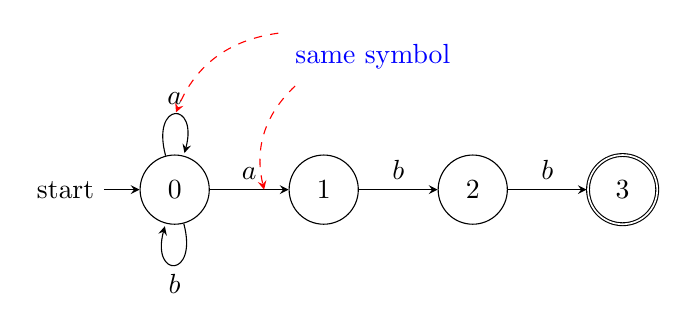
\begin{tikzpicture}[auto,
    ->,
    >=stealth
  ]
    \node[initial, state]   (0)                {$0$};
    \node[state]            (1) [right = of 0] {$1$};
    \node[state] (2) [right = of 1] {$2$};
    \node[state, accepting] (3) [right = of 2] {$3$};
    
    \path (0) edge[loop above] node {$a$} (0)
          (0) edge[loop below] node {$b$} (0)
          (0) edge node {$a$} (1)
          (1) edge node {$b$} (2)
          (2) edge node {$b$} (3)
    ;

\pause
	\node[jn, above=0.5cm of 0] (j1) {};
	\node[inv, above right=of 0] (l1) {\color{Blue}same symbol};
	
	\draw[->, Red, dashed, bend right] (l1) to (j1);
	
	\coordinate(e1) at ($(0)!0.6!(1)$);
	\draw[->, Red, dashed, bend right] (l1) to (e1);
  \end{tikzpicture}
}

\end{center}
\pause
\textbf{Language:} \pause$(a|b)\star abb$


\end{frame}
% frame end %%%%%%%%%%%%%%%%%%%%%%%%


% frame begin %%%%%%%%%%%%%%%%%%%%%%%%
\begin{frame}{Non-Deterministic FSA (NFA)}
\myminorheader{Example 2}
\begin{center}
\resizebox{0.4\textwidth}{!}{%
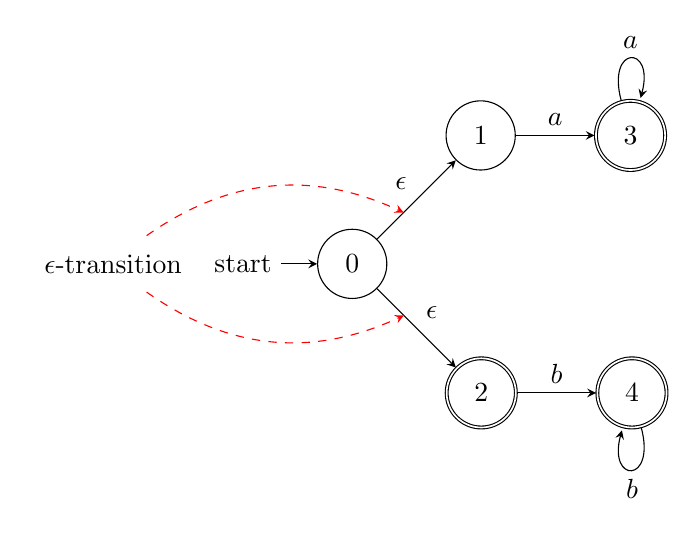
\begin{tikzpicture}[auto,
    ->,
    >=stealth
  ]
    \node[initial, state]   (0)                {$0$};
    \node[state]            (1) [above right = of 0] {$1$};
    \node[state, accepting] (2) [below right = of 0] {$2$};
    \node[state, accepting] (3) [right = of 1] {$3$};
    \node[state, accepting] (4) [right = of 2] {$4$};
    
    \path (0) edge node {$\epsilon$} (1)
          (0) edge node {$\epsilon$} (2)
          (1) edge node {$a$} (3)
          (2) edge node {$b$} (4)
          (3) edge[loop above] node {$a$} (3)
          (4) edge[loop below] node {$b$} (4)
          
    ;
\pause
	\node[inv, left=1.5cm of 0](l1){$\epsilon$-transition};
	\coordinate(e1) at ($(0)!0.4!(1)$);
	\coordinate(e2) at ($(0)!0.4!(2)$);
	\draw[->, Red, dashed, bend left] (l1) to (e1);
	\draw[->, Red, dashed, bend right] (l1) to (e2);
    
  \end{tikzpicture}
}

\end{center}
\textbf{Language:} $aa\star|bb\star$

\end{frame}
% frame end %%%%%%%%%%%%%%%%%%%%%%%%

% frame begin %%%%%%%%%%%%%%%%%%%%%%%%
\begin{frame}{Non-Deterministic FSA (NFA)}
\begin{itemize}
	\item Finite set of states -- ($S$)
	\item Alphabet - ($\sum$)
	\item Transition function ($T : S \times \sum \rightarrow 2^S$)
	\item Initial state ($S_0$)
	\item Final/accepting states ($F \subseteq S$)
	\pause
	\item \textbf{Acceptance of a string: }When there exists a path corresponding to the input leading to an accepting state.
\end{itemize}

\pause
\myminorheader{Specific Properties}
\begin{itemize}
	\item The same state can transition to more than one states on the same symbol
	\item $\epsilon$-transitions
\end{itemize}

\end{frame}
% frame end %%%%%%%%%%%%%%%%%%%%%%%%

% frame begin %%%%%%%%%%%%%%%%%%%%%%%%
\begin{frame}{Deterministic FSA (DFA)}
\begin{itemize}
	\item Finite set of states -- ($S$)
	\item Alphabet - ($\sum$)
	\item Transition function ($T : S \times \sum \rightarrow S$)
	\item Initial state ($S_0$)
	\item Final/accepting states ($F \subseteq S$)
	\item \textbf{Acceptance of a string: }When there exists a path corresponding to the input leading to an accepting state.
\end{itemize}

\pause
\myminorheader{Specific Properties}
\begin{itemize}
	\item Only one next-state on the same symbol
	\item No $\epsilon$-transitions
\end{itemize}

\end{frame}
% frame end %%%%%%%%%%%%%%%%%%%%%%%%

% frame begin %%%%%%%%%%%%%%%%%%%%%%%%
\begin{frame}{Deterministic FSA (DFA)}

\myminorheader{Example 1}

\begin{center}
\resizebox{!}{0.2\textheight}{%
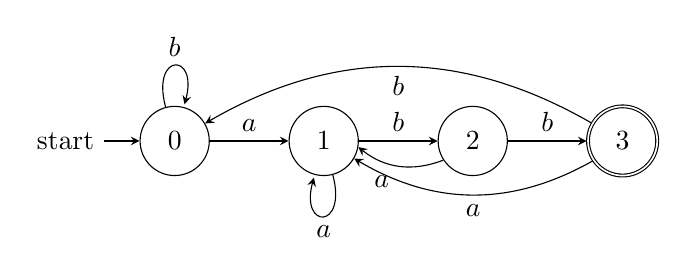
\begin{tikzpicture}[auto,
    ->,
    >=stealth
  ]
    \node[initial, state]   (0)                {$0$};
    \node[state]            (1) [right = of 0] {$1$};
    \node[state] (2) [right = of 1] {$2$};
    \node[state, accepting] (3) [right = of 2] {$3$};
    
    \path (0) edge[loop above] node {$b$} (0)
          (0) edge node {$a$} (1)
          (1) edge[loop below] node {$a$} (1)
          (1) edge node {$b$} (2)
          (2) edge node {$b$} (3)
          (2) edge[bend left] node {$a$} (1.350)
          (3) edge[bend left] node {$a$} (1.330)
          (3) edge[bend right] node {$b$} (0)
    ;
    
  \end{tikzpicture}
}

\end{center}
\pause
\textbf{Language:} \pause$(a|b)\star abb$


\end{frame}
% frame end %%%%%%%%%%%%%%%%%%%%%%%%

% frame begin %%%%%%%%%%%%%%%%%%%%%%%%
\begin{frame}{NFA and DFA}
\begin{itemize}
	\item NFAs: Often more readable
	\item NFAs: Usually have fewer states
	\pause
	\item DFAs: Less readable
	\item DFAs: Larger number of states
	\item DFAs: Faster to simulate
	\pause
	\item Equally expressive $\equiv$ Regular expressions (Regular languages)
\end{itemize}
\end{frame}
% frame end %%%%%%%%%%%%%%%%%%%%%%%%

% frame begin %%%%%%%%%%%%%%%%%%%%%%%%
\begin{frame}{Lexical Analysis Process}
\begin{center}
\resizebox{0.7\textwidth}{!}{%
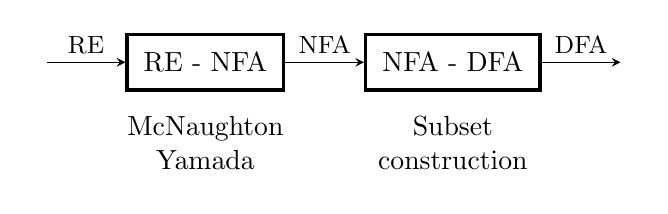
\begin{tikzpicture}[auto,
    ->,
  %  shorten >=2pt,
    >=stealth,
  %  node distance=1cm,
    bb/.style={%
      rectangle, draw=black, very thick, fill=white,
      text ragged, minimum height=2em, inner sep=6pt, align=center
    },
]
    \node      (0)                {};
    \node[bb]  (1) [right = of 0] {RE - NFA};
    \node[bb]  (2) [right = of 1] {NFA - DFA};
    \node      (3) [right = of 2] {};
    \node[inv]  (l1) [below = 0.1cm of 1] {McNaughton \\ Yamada};
    \node[inv]  (l1) [below = 0.1cm of 2] {Subset \\ construction};
\begin{small}
    \path (0) edge node[align=center] {RE}  (1)
          (1) edge node[align=center] {NFA} (2)
          (2) edge node[align=center] {DFA} (3)
    ;
\end{small}
  \end{tikzpicture}
}

\pause

\begin{tikzpicture}
\node[rectangle, draw=Red, fill=Red]{};
\end{tikzpicture}
\end{center}

\end{frame}
% frame end %%%%%%%%%%%%%%%%%%%%%%%%


% frame begin %%%%%%%%%%%%%%%%%%%%%%%%
\begin{frame}{Next}
\myheader{Simulation of FSAs}
\end{frame}
% frame end %%%%%%%%%%%%%%%%%%%%%%%%
\end{document}
